\documentclass[review]{elsarticle}
%\documentclass[final,times,letterpaper,12pt]{elsarticle}

\usepackage{lineno}
\usepackage{graphicx} 
\usepackage{subcaption}
\usepackage{amsmath}
\usepackage{booktabs}
\usepackage{float}
\usepackage[unicode=true]{hyperref}


\usepackage[dvipsnames]{xcolor} % Für Einfärbung von Notizen. Sollte am Ende wieder entfernt werden.

\modulolinenumbers[5]

%\usepackage{etoolbox}
% \patchcmd{<cmd>}{<search>}{<replace>}{<success>}{<failure>}
%\patchcmd{\emailauthor}{(#2)}{}{}{}
\patchcmd{\urlauthor}{(#2)}{}{}{}

\journal{Journal of PLACEHOLDER}


%%%%%%%%%%%%%%%%%%%%%%%
%% Elsevier bibliography styles
%%%%%%%%%%%%%%%%%%%%%%%
%% To change the style, put a % in front of the second line of the current style and
%% remove the % from the second line of the style you would like to use.
%%%%%%%%%%%%%%%%%%%%%%%

%% Numbered
%\bibliographystyle{model1-num-names}

%% Numbered without titles
%\bibliographystyle{model1a-num-names}

%% Harvard
%\bibliographystyle{model2-names.bst}\biboptions{authoryear}

%% Vancouver numbered
%\usepackage{numcompress}\bibliographystyle{model3-num-names}

%% Vancouver name/year
%\usepackage{numcompress}\bibliographystyle{model4-names}\biboptions{authoryear}

%% APA style
\bibliographystyle{model5-names}
\biboptions{authoryear}

%% AMA style
%\usepackage{numcompress}\bibliographystyle{model6-num-names}

%% `Elsevier LaTeX' style
%\bibliographystyle{elsarticle-num}
%%%%%%%%%%%%%%%%%%%%%%%

\begin{document}

\begin{frontmatter}

\title{The Role of Media Coverage in Shaping Household Inflation Expectations: An Analysis of ECB Press Conferences and News Reporting}

\author {Jasper Bär\corref{cor1}}
\ead{ja.baer@stat-econ.uni-kiel.de}
\ead[url]{PLACEHOLDER Github url}

\cortext[cor1]{PLACEHOLDER}

\begin{abstract}
PLACEHOLDER Abstract
\end{abstract}

\begin{keyword}
PLACEHOLDER Keyword 1 \sep Keyword 2 \sep Keyword 3 \sep Keyword 4 \sep Keyword 5
\end{keyword}

\newpageafter{abstract}

\end{frontmatter}

\newpage

\section{Introduction} \label{sec:intro}

%Hook/Attention-grabber (existiert)
%Background and context (existiert, aber noch lückenhaft und muss besser zusammengefügt werden)
%Gap in the literature (existiert, anders in den Text einfügen?)
%Research question or objective (existiert)
%Scope and limitations (fehlt noch)
%Methodological approach (existiert)
%Significance and contribution (existiert)
%Roadmap/Outline (wegglassen?)

% Hook 
Central bank communication has become a vital instrument in modern monetary policy \citep{Blinderetal2017}. Central banks use communication as a tool for guiding inflation expectations and ensuring trust in their monetary policy. Historically, much of this communication has been directed towards financial experts. However, in recent years, central banks have increasingly been reaching out to the general public \citep{Blinderetal2022}. The media plays a critical role in this process by disseminating central bank communication to a broader audience. Therefore, it is essential to understand how the media reports on central bank communication to analyze the impact of central bank communication on the general public.
%
% Background and context
%
% Literature on inflation expectations
% Literature on Media impact on expectations
%
\\
Since \cite{Carroll2003} created a model for inflation expectations that considers the amount of media coverage, several studies have analyzed the role of media coverage for the inflation expectation forming process. \cite{Draeger2015} find a small effect of media on inflation expectations and perception for Sweden. Similarly, \cite{LamlaLein2014} find that media reporting influences the accuracy of German household inflation expectations. \citep{Larsen2021} show that the news topics also have predictive power for inflation expectations. \cite{Ehrmann2017} show that increased media coverage leads to the strongest improvements in inflation expectations accuracy during recessions and for individuals with pessimistic views or financial difficulties.  
%\cite{Jansen2018} however find that more freuqent readership of popular newspapers is assoziated the less inflation perception accuracy for Dutch households. 
%
% Literature on central banks impact on household inflation
%
\\
% "Fed speak on main street: Central bank communication and
% household expectations" has good literature overview for this section.
%
Another recent branch of the literature investigates the impact of central bank communication on household inflation expectations. \cite{Coibion2022} show that the Fed's communication can have a significant effect on the household's inflation expectations when the communication is directly presented to the households. However, the effect of the communication is significantly damped when the same information is presented in the form of newspaper articles. This view is in line with \cite{Gardt2022} who demonstrate that households mostly hear about the ECB's monetary policy through television and newspapers (online and printed) and rarely by using direct sources like the ECB website. Similarly, \cite{LamalaVinogradov2019} find that FOMC announcements have no impact on consumers' inflation perception and expectation, but that FOMC announcements increase the probability of consumers to receive news about the FOMC announcements. 
%
% Literature on Central banks in media
%
\\
Several studies investigate how central bank communication is perceived by the media. \cite{Berger2011} and \cite{Picaultetal2022} show that the media's assessment of ECB policy decision is highly responsive to the content of ECB press conferences. %More citations?
%
% Gap in the literature
%
\\
Similar to \cite{Picaultetal2022}, I adopt a framework proposed by \cite{HayoNeuenkirch2015} where the media acts as a channel between central bank communication and the perception of monetary policy by financial markets. Following \cite{Nimark2019} who formalize that agents delegate their information choice to the media rather than monitor all relevant events themselves. Hence, news act as a channel through which households receive information about the central bank communication. Building on these two frameworks, I assume that the media coverage of central bank communication acts as a channel between the central bank and households. I assume that households consume the news from the media about the central bank communication rather than directly from the central bank communication itself. 
%
%This view gets supported by a number of survey-based studies indicating that household are often poorly informed about monetary policy and the objectives of their respective central banks. \cite{Cruijsenetal2015} show that Dutch households understanding about the ECB's objectives are poor. Similar most German \citep{HayoNeuenkirch2018} and Italian \citep{Bottonetal2021} households do not know that the main objective of the ECB is to maintain price stability in the euro zone. However, \cite{Cruijsenetal2015} and \cite{HayoNeuenkirch2018} show that people who receive their information about monetary policy via television and newspapers are better informed their central bank and monetary policy.\textcolor{red}{(To close to Blinder et al. 2022)}
%
% Research Question
%
\\
I am examining the impact of media coverage in newspapers on households' inflation expectation accuracy, specifically focusing on reporting of ECB press conferences and news about inflation. Firstly, I explore whether the inflation information presented in newspapers deviates from the inflation information in the press conferences by the ECB. Secondly, I investigate the extent to which the deviation of inflation information in media coverage and ECB press conferences contributes to explaining the errors in households' inflation expectations.
%
% Scope and limitations
%
%The newspaper data consists of over 6 million German articles ranging from the 1. January of 2002, the day of the introduction of Euro banknotes and coins in Germany, until 31. of December 2018\footnote{The Euro was already introduced as book money in Germany on 1. January 1999.}. The ECB press conference are publicaly available on the official ECB website.
%\\
%
% Significance and contribution
%
\\
This paper is, to my knowledge, the first to explicitly investigate the link between central bank communication and news coverage concerning household inflation expectations. Furthermore, it contributes to the literature by demonstrating how news about inflation deviates from the corresponding ECB communication, allowing for a better understanding of how central bank communication is conveyed to the general public and explaining the channel through which the general public reacts to central bank communication.
%
%Methodological approach
%
\\
I built on the Bayesian learning model \citep{LamlaLein2014} to examine the impact of the difference between inflation related information in media reporting and ECB press conferences on household's inflation expectations accuracy. To quantify the inflation related information in the ECB press conferences and news, I apply the lexicon driven procedure by \cite{PicaultRenault2017} to create lexicons for inflation related information for the news and for the ECB press conferences. To measure how closely the media follows ECB press conferences in their news, I apply a similar procedure as \cite{Picaultetal2022} and use dependency parsing to identify the grammatical structure of a text and filter out the share of news that reproduce ECB press conferences from general news about inflation. This allows me to measure how closely the media reporting follows the ECB's press conferences.
%
% Teaser Results
%
\\
I find that the inflation information in both news and ECB press conferences shares a strong correlation with the current inflation rate in Germany. Moreover, the discrepancy in inflation reporting between news and ECB press conferences exhibits a significant correlation with the gap in inflation expectations between German households and professional inflation forecasts.
%nochmal nachprüfen
%However, \cite{Picaultetal2022} and \cite{Cruijsenetal2015} note that the perception of financial markets is simultaneously influenced by the central bank communication and the media coverage of the corresponding events and central bank communication.
%A small but rapidly growing branch of the literature focuses on central bank communication, i.e., the information provided by central banks to the general public, and its connection to different variables of interest like financial variables or future monetary decisions of the central bank. For example, \cite{PicaultRenault2017} show that ECB press statements can be used to predict future ECB monetary decisions. \textcolor{red}{(Give more examples)}
%A subbranch of this literature focuses on the connection between inflation expectations and central bank communication. \cite{Picaultetal2022} investigate how the reporting about the ECB in the media can be used to predict financial market inflation expectations. \\
% Kurzer Abschnitt in der ich auf Media Biases eingehe (Media reacts to central bank communication, negativity bias)
\section{Model}\label{sec:Model} 
I extend the Bayesian learning model for inflation expectation by \cite{LamlaLein2014} by explicitly adding a channel for central bank communication. I assume that the central bank sends a noisy signal for the future inflation $\pi_{t+1}$ 
%based on the observation of variables which are relevant for the inflation $\mathbf{X}_t$ to the media
.Let $c_t$ denote the signal that captures information about the central bank's inflation forecast $\Theta_t$ that the central bank communicates to the media; that is, inflation-related information in press conferences. I further assume that the signal is normally distributed, $c_t \sim N(\Theta_t, \sigma^c_t)$, with variance $\sigma^c_t$. This assumption implies that the central bank only sends one unambiguous signal at each period $t$ rather than multiple conflicting signals at the same period.
% In the case of the ECB this inflation forecast is equal to the ECB staff's inflation projection 
%\\
%$ c_t = \pi_{t+1} + \epsilon_t \quad \epsilon_t \sim N(0, \sigma^c_t)$
%\\ 
%where $\epsilon_t$ represents the noise in the central bank's observation. 
%\\
In the absence of the central bank's communication, the media sends a noisy "baseline" signal about the rational forecast of inflation $\Psi_t$ for future inflation $\pi_{t+1}$ to households based on a number of media reports $V$, with $s^b_{\nu,t} \sim N(\Psi_t + \alpha_t, \sigma^{sb}_t)$. Here, $\alpha_t$ captures the media bias, and I assume that $\alpha_t > 0$. The media can decide how closely to follow the central bank's communication. Therefore, the media's inflation signal can be defined as:
\begin{equation}
s_{\nu,t} = (1-\lambda_{\nu,t}) s^b_{\nu,t} + \lambda_{\nu,t} c_t \quad 0\leq \lambda_{\nu,t} \leq 1
\end{equation}
where $\lambda_{\nu, t}$ denotes the weight that the media report places on the central bank's signal $c_t$ relative to the "baseline" media signal $s^b_{\nu,t}$. A value of $\lambda_{\nu,t} = 0$ indicates that the media report completely ignores the central bank's communication, while $\lambda_{\nu,t} = 1$ describes a situation where the media only reproduces information from the central bank's communication.
\\
Given that $s_{\nu,t}$ is a linear combination of normal random variables and assuming that $\sigma^c_t$ and $\sigma^{sb}{\nu,t}$ are independent, the media sends a normally distributed signal about $\pi{t+1}$ with $s_{\nu,t} \sim N(\mu^s_{\nu,t}, \sigma^s_{\nu,t})$, where:
\begin{equation} 
\mu_{\nu,t}^s = (1-\lambda_{\nu,t}) (\alpha_t + \Psi_t) + \lambda_{\nu,t} \Theta_t 
\end{equation}
\begin{equation}
\sigma_{\nu,t}^s = \lambda_{\nu,t}^2 \sigma_{\nu,t}^{s^b} + (1- \lambda_{\nu,t})^2 \sigma^c_{\nu,t}
\end{equation}
%\begin{equation}
%\mu_s = \lambda_t \alpha_t + \pi_{t+1} 
%\end{equation}
\\
The households hold a prior belief $\gamma_t \sim N(\pi_t, \sigma^h_t)$ about the future inflation $\pi_{t+1}$. The households then update their beliefs based on the media's signal. Following the Bayesian updating rule, the households' posterior beliefs about future inflation $\pi_{t+1}$ are:
\begin{equation}
\pi_{t+1}^h \sim N(\mu^h_{t+1}, \sigma^h_{t+1})
\end{equation}
where $\mu^h_{t+1}$ and $\sigma^h_{t+1}$ are the updated mean and variance of the household's belief about future inflation, respectively. To compute the updated mean and variance, the households combine their prior beliefs with the media's signal:
%\begin{equation}
%\mu^h_{t+1} = \frac{\sigma^s_{\nu,t} \gamma_t + \sigma^h_t \mu^s_{\nu,t}}{\sigma^s_{\nu,t} + \sigma^h_t}
%\end{equation}
%\begin{equation}
%\sigma^h_{t+1} = \frac{\sigma^s_{\nu,t} \sigma^h_t}{\sigma^s_{\nu,t} + \sigma^h_t}
%\end{equation}

%Hence, the representative household forms its inflation expectations according to
%%\begin{equation}
%%f(\pi_{t+1}|c_t, \pi_t, \lambda_{\nu,t}, \alpha_{\nu,t}) \propto \Pi^V_{\nu = 1} h(s_{\nu,t}|\alpha_{\nu,t}, \pi_t, \lambda_{\nu,t}) k(\pi_t)
%%\end{equation}
%\begin{equation}
%f(\pi_{t+1}|s_{\nu,t}) \propto \Pi^V_{\nu = 1} h(s_{\nu,t}|\alpha_t, \Psi_t, \lambda_{\nu,t}, \Theta_t) k(\pi_t)
%\end{equation}
%
%where $f(.)$ is the posterior belief of a representative household on inflation $\pi_{t+1}$ after receiving the inflation related news signal. Assuming normality the posterior distribution is a normal distribution with mean $\mu_t$

\begin{equation}
\mu_t = \rho_t \pi_t + (1- \rho_t) \bar{\mu_t^s} 
\end{equation}
where
\begin{equation}
\bar{\mu_t^s} = V^{-1} \sum^V_{\nu = 1} \mu_{\nu,t}^s = V^{-1} \sum^V_{\nu =1} (1-\lambda_{\nu,t}) (\alpha_t + \Psi_t) + V^{-1} \sum^V_{\nu =1} \lambda_{\nu,t} \Theta_t  
\end{equation}
\begin{equation}
=\Psi_t + \alpha_t - \bar{\lambda_t} \alpha_t - \bar{\lambda_t} \Psi_t + \bar{\lambda_t}\Theta_t 
\end{equation}
\begin{equation}
=\bar{\lambda_t}(\Theta_t - \Psi_t) + \alpha_t(1- \bar{\lambda_t}) + \Psi_t
\end{equation}
and
\begin{equation}
\rho_t = \frac{\frac{1}{V}\sigma^s_t}{{\sigma^h_t + \frac{1}{V}}\sigma^s_t}
\end{equation}
\\
For $\bar{\lambda_t} = 0$, the mean would be $\mu_t = \rho_t \pi_t + (1- \rho_t) (\alpha_t + \Psi_t)$. Hence, if the media completely ignores the central bank communication, the mean of the posterior is the weighted average of the prior and the biased media signal\footnote{This case is equivalent to the model from \cite{LamlaLein2014} with media bias.}. If the media perfectly reproduce the central bank communication, i.e., $\bar{\lambda_t} = 1$, the mean would be $\mu_t = \rho_t \pi_t + (1-\rho_t) \Theta_t$. 
\\
$B_t$ is the difference between the professional inflation forecast and the household inflation expectations. I assume that the rational inflation forecasts of the central bank and of the media are similar, i.e, $\Theta_t \approx \Psi_t$.
\begin{equation}
B_t = |\mu_t - \Psi_t| = |\rho_t \pi_t + (1-\rho_t)(\alpha_t(1- \bar{\lambda_t}) + \Psi_t) - \Psi_t|
\end{equation}
\begin{equation}
= |\rho_t (\pi_t - \Psi_t - \alpha_t (1-\bar{\lambda}_t)) + \alpha_t (1- \bar{\lambda}_t)|
\end{equation}
\begin{equation}
= |(1-\rho_t)(1-\bar{\lambda}_t)\alpha_t + \rho(\pi_t - \Psi_t)|
\end{equation}
\\
If $\pi_t$ is larger or close to $\Psi_t$ 
\begin{equation}
= (1-\rho_t)(1-\bar{\lambda}_t)\alpha_t + \rho(\pi_t - \Psi_t) > 0
\end{equation} 
\begin{equation}
\frac{\partial B_t}{\partial \bar{\lambda_t}} = -(1-\rho_t)\alpha_t < 0
\end{equation}
Hence, an increase in $\lambda_t$ will lead to a decrease in the inflation expectation error of the households. The intuition behind this is that if the prior inflation $\pi_t$ is considerably larger or close to the rational forecast $\Psi_t$, households may overshoot their expectations based on their prior. Consequently, increasing the weight given to the central bank communication helps to adjust the expectations downward.
\\
Similar, for $\pi_t <<\Psi_t$
\begin{equation}
= (1-\rho_t)(1-\bar{\lambda}_t)\alpha_t + \rho(\pi_t^0 - \Psi_t) < 0
\end{equation}
\begin{equation}
\frac{\partial B_t}{\partial \bar{\lambda_t}} = (1-\rho_t)\alpha_t > 0
\end{equation}
If the prior inflation $\pi_t$ is significantly smaller than $\Psi_t$, households undershoot their inflation expectations. In this case, the effect of an increase in $\lambda_t$ increases the expectation error if the media bias is positive, as the media bias acts as an upward "correction." The more weight the media places on their baseline signal, the larger the effect of $\alpha_t$, which then corrects the inflation expectations upward.
\\ 
Thus, the partial effect of the weight given to the central bank increases the inflation forecast accuracy is ambiguous and depends on the size of $\pi_t$ and $\Psi_t$. The effect is stronger, the larger the media bias is. 
\\
The weight determines how closely the media follows their "baseline" signal. The "baseline" signal introduces the media bias into the overall media signal. Therefore, the closer the media follows their "baseline", the stronger the media bias in the overall media signal. 
From this follows my first hypothesis
\par
\textbf{Hypothesis 1:} \textit{If the media's signal is affected by a media bias, an increase in the weight given to the central bank communication by the media has an ambiguous effect on the household inflation forecasting accuracy, depending on the size of the difference between the current inflation and the rational inflation forecast.} 
\par
Similarly, the media bias can affect the inflation forecasting accuracy of households. The partial effect of the media bias for $\pi_t$ larger or close to $\Psi_t$ is
\begin{equation}
\frac{\partial \mathbf{B}_t}{\partial \alpha_t} = (1-\rho_t) (1-\bar{\lambda_t}) > 0 
\end{equation}
and for $\pi_t << \Psi_t$
\begin{equation}
\frac{\partial \mathbf{B}_t}{\partial \alpha_t} = -(1-\rho_t) (1-\bar{\lambda_t}) < 0 
\end{equation}
The sign of the partial effect of the media bias is ambiguous, depending of the difference between $\Psi_t$ and $\pi_t$. The media bias can either bias the expectations upward for $\pi_t$ larger or close to $\Psi_t$, or "correct" the expectations if the prior is sufficiently small. The size of the effect is determined by $\lambda_t$.  A high weight of the media's "baseline" signal increases the size of effect of the media bias has on the overall media signal. 
Hence, my second hypothesis is
\par
\textbf{Hypothesis 2:} \textit{An increase of the media bias by the media has an ambiguous effect on the household inflation forecasting accuracy depending on the size of the difference between the current inflation and the rational inflation forecast.}
%\\
%\textcolor{red}{Additional hypothesis 3 - (WIP)}
%\\
%I assume that the households prior variance $\sigma^h_t$ depends positively on the economic uncertainty $U_t$, $\frac{\partial \sigma^h_t}{\partial U_t}$, while the medias "baseline" signal and central banks communication signals are not affected by the economic uncertainty. Hence, $\frac{\partial \rho_t}{\partial U_t} < 0$.  
%\\
%\textcolor{red}{Additional hypothesis 4 - (WIP)}
%\\
%\\
%\textbf{Hypothesis 3:} \textit{The households place a higher weight on the media signal during periods of economic uncertainty or high inflation.}
%\\
%\textcolor{red}{This would be an interesting hypothesis, but it is currently not in the model. Maybe I could link higher uncertainty to an increase in $\sigma^h_t$. I should also double check \cite{LamlaLein2014} for that.}
%\\
%\textbf{Hypothesis 4:} More transparent central bank communication reduces the inflation expectation bias.
%\\
%\textcolor{red}{This would be an interesting hypothesis, but it is currently not in the model.}
%\textcolor{red}{Note: For a robustness check I could assume that households directly observe the ECB communication. Maybe I could create a scenario in which the household ignore the media and only receive a news signal from the ECB, simulating a "perfect" communication scenario for the ECB.}  

\section{Data} \label{sec:Data}

My dataset consists of two distinct components: textual data from ECB press conferences and newspaper articles, and quantitative data on inflation and inflation expectations. Section~\ref{sec:Textual_Data} describes the textual data, and Section~\ref{sec:Quantitative_Data} outlines the quantitative data.

\subsection{Textual Data} \label{sec:Textual_Data}

I collected two separate datasets for textual analysis: one for ECB communications and another for newspaper articles. The ECB's primary mode of communication with the media is through their press conferences, which are conducted in English every six weeks following the ECB's Governing Council monetary policy decisions. I gathered ECB press conference transcripts from the official ECB website from 2000 to 2022 using a web scraper. I excluded the Q\&A section and other less significant sections, such as greetings and acknowledgments, retaining only the introductory statements.
%\textcolor{red}{Ich sollte um Erlaubnis fragne, sonst sagen, dass die Presse Conferenzen manuell gesammelt wurden.} 
% \textcolor{red}{(cite other who done it similarly?)}.
\\
The media news data was provided by Dpa, the largest German news agency. This dataset consists of over 7 million newspaper articles in German published by Dpa between 1991 and 2018. I filtered out articles unrelated to the economy and those solely focused on financial news, such as stock movement reports or business updates. Furthermore, I removed purely numeric information like tables from the articles. For a detailed description of the cleaning process, see \textcolor{red}{[Cite Mariia, Philip, Kai, and me]}.
\\
To isolate data relevant to inflation, I included only sentences containing the word "Inflation" and its synonyms, such as "Preisteigerung" or "Preiserhöhung" (price increase) \footnote{The words are: Inflation (Inflation), Inflationsrate (Inflation rate), Verbraucherpreisindex (Consumer Price Index, CPI), Lebenshaltungskosten (Cost of living), Geldentwertung (Currency devaluation), Teuerung (Price inflation), Preisanstieg (Price increase), Preiserhöhung (Price hike), Verteuerung (Increase in prices), Deflation (Deflation), Hyperinflation (Hyperinflation), Geldwert (Money value), Preisindex (Price index), Preisniveau (Price level), Kaufkraft (Purchasing power), and Warenkorb (Basket of goods).}.
\\
To reduce the dimensionality of the remaining data, I applied several pre-processing steps commonly used in the literature to both textual datasets: lowercasing, removing punctuation, eliminating stopwords (e.g., and, but, or) that convey no information, and removing numbers.
%\textcolor{red}{(better word?)}. 
%I futhermore ensure that all duplicates \textcolor{red}{Add further steps which we take}. 
%\\
%\textcolor{red}{Note 1: I need to double check with Kai if I'm allowed to even use the dpa data or I'm limited to the LexisNexis data which would be considerable smaller.}
%\\
%\textcolor{red}{Note 2: News dataset is in German, ECB dataset in English}
%\\
%\\
%\textcolor{red}{Note 4: Not sure if this is the best way to select inflation related sentences. Maybe some kind of topic modeling would be better suited.}

\subsection{Quantitative Data} \label{sec:Quantitative_Data}

I use the quarterly year-on-year HICP growth rate for Germany, sourced from the Eurostat database, as a measure of inflation.
\\
For the rational inflation forecast, I employ the ECB surveys of professional forecasters. Each quarter, the ECB surveys professional forecasters about their year-on-year inflation expectations. To obtain the final forecast, I calculate the average of all forecasts. The survey data covers the period from the first quarter of 1999 to the last quarter of 2022.
\\
For household inflation expectations, I utilize the monthly European Commission's Business and Consumer Survey. In this survey, German households are asked about their expectations regarding price changes in the next 12 months. They can anticipate faster rising prices, prices rising at a consistent pace, prices rising more slowly, prices remaining unchanged, or prices decreasing.
\\
To transform qualitative survey responses into quantitative inflation expectations, I apply a rolling-window regression-based approach by \cite{Lahiri2015}. This approach is based on an extended version of \cite{Carlson1975} by \cite{Berk1999} and has been simplified by \cite{Rosenblatt-Wisch2015}. A detailed explanation can be found in Section \ref{sec:Quantification_of_Inflation_Expectations}.
\\
Although quantifying qualitative survey data is not as optimal as using quantitative survey results, it is necessary due to the lack of publicly available quantitative survey-based inflation expectations data for German households.
%\textcolor{red}{Cite others who also done it like that}
%\\
%\textcolor{red}{NOTE: Change window size.}
\section{Text Classification} \label{sec:Quantification of Text Data}
In this section, I explain my methodology for quantifying ECB communication and newspaper articles. I divide my dataset into individual sentences and classify each sentence according to predefined categories. ECB press conferences fall into three categories, each consisting of three classes. The first two categories, adapted from \cite{PicaultRenault2017}, characterize the monetary stance as monetary hawkish, monetary neutral, or monetary dovish, and represent the economic outlook as positive, neutral, or negative. I introduce a third category that conveys the inflation outlook as increasing, steady, or decreasing, enabling a direct comparison between inflation expectations communicated in ECB press conferences and those expressed in the news media.
\\
News articles are classified into two categories, each with three classes. The first category describes the economic impact of inflation reported in the news as positive, neutral, or negative, while the second category indicates the direction of inflation as increasing, neutral, or decreasing.
%\textcolor{red}{Note 1: Is it obvious enough why I used two different training datasets?}
%\\
%\textcolor{red}{I should further describe my annotation scheme in the appendix and give some examples.}
\\
To achieve the text classification two main approaches are used in the literature: Machine Learning text classification and Lexicon-based text classification. Machine Learning (ML) text classification utilizes complex probabilistic models, usually trained on large datasets. Modern ML models are able to take into account the grammatical and syntactical structure of texts. However, the complexity of these models comes with a drawback. Modern deep-learning models like BERT (Devlin et al 2018) are "black-boxes" and require large training datasets.
\\
Lexicon-based text classification utilizes a lexicon to classify the category of a given text. A lexicon is a collection of words or phrases associated which specific category classes. This approach relies on the frequency, or weights of the words or phrases in the lexicon to determine the category of a given text. 
\\
The simple implementation and transparency of Lexicon-based sentiment classification has made it widely used in the economic and finance literature, e.g., \cite{Shapiro2022}, \cite{Loughran2011}, \cite{Barbaglia2022}, \cite{Nyman2021}, \cite{Ardia2019}. The most prominent lexicon for sentiment classification of texts from the finance and economic domain was created by \cite{Loughran2011}). \cite{PicaultRenault2017} developed a lexicon for classifying ECB press conferences and measuring the conveyed economic outlook and monetary stance . However, these lexicons were not created for classifying inflation directions and sentiment with regard to inflation. Hence, I implement a similar approach like \cite{Shapiro2022} and \cite{PicaultRenault2017} and create data-driven lexicons based on the training datasets created by me. The lexicon is then used to classify each sentence in the ECB press conferences according to the three mentioned categories and each of the newspaper sentences according to the two mentioned categories.
\\
I created two training datasets: one for the newspaper articles and one for the ECB press conferences. Due to the different categories and different styles of these two types of text, I created two training datassets.
\\
I manually classified 3000 randomly drawn sentences from the ECB press conferences according to the three categories, with each sentence being labeled with one of the three classes for each category. Similarly, 3000 sentences were randomly drawn from the news corpus and labeled based on the two categories. I then used these datasets to create one lexicon for the ECB press conferences and for the newspaper articles.
\\
The lexicons are created by calculating the degree to which each word in the training dataset is associated with a class. The association is calculated using pointwise mutual information (PMI). Following Church and Hanks (1990) PMI is defined as
\begin{equation}
PMI(c,w) = log_2 (\frac{p(c,w)}{p(c)p(w)})
\end{equation}
where $p(w)$ is the words share of total words in the training dataset, $p(c)$ is the total share of sentences belonging to class $c$ and $p(c,w)$ is the words share in class $c$ of total words. The PMI measure how closely a is associated with a class. This formula is applied to all words for all categories in the two training datasets.  
\\
The lexicons are then used to to assign a category specific score to each press conference and newspaper sentences. Each ECB press conference is treated as a independent text and all newspapers sentences from one month are concatenated to one text for each month. Then I calculate a score for each category and score by.
\begin{equation}
score_i^c = \frac{\sum_{j=1}^n (PMI(c_3, w_{i,j}) - PMI(c_1,w_{i,j}))}{\sum_{j=1}^n (PMI(c_3, w_{i,j}) + PMI(c_2, w_{i,j}) + PMI(c_1, w_{i,j}))}
\end{equation}
where $score_i^c$ is the score of text $i$ specific to category $c_g$. $g$ denotes the class in the respective category.For the ECB monetary categories these are $c_3$ for hawkish, positive economic outlook and increasing inflation. $c_1$ stands for dovish, negative economic outlook and decreasing inflation. $c_2$ denotes the neutral class. For the newspaper data $c_3$ stand for increasing inflation and positive sentiment. $c_1$ for decreasing inflation and negative sentiment. $PMI(c_3, w_{i,j})$, $PMI(c_2, w_{i,j})$, and $PMI(c_1, w_{i,j})$ are the PMI values of word $w_{i,j}$ in text $i$ of the respective class, and $n$ is the number of words in the text. 
\\
To improve the text classification, I follow \cite{Shapiro2022} and implement negations. Negation words like "not" directly impact the class of a sentence, e.g., "the inflation is rising" vs. "the inflation is not rising". I follow CITE and handle these negations by multiplying the PMI-value of each word by $-1$ if the word is within a three word window of a negation word. 
\\
For the newspaper articles, I have therefore two monthly indizes. One for the direction of the inflation and one for the sentiment regarding the inflation. I combine both these indizes to one by multiplying them with each other. I call the resulting index Inflation News Index (INI). 
\\
The (ECB) press conferences, occur eight times a year. To convert the press conference-based indizes to a monthly frequency, I create a monthly time series covering the entire period for which I have press conference data. For each month, I assign the index value from the most recent press conference preceding that month. This approach assumes that the index remains constant between press conferences and only changes when a new press conference is released. By using this method, I obtain a monthly index that reflects the information available to market participants at each point in time. 
%\textcolor{red}{I further deviate from Picault et. al (2017) or similar papers like Marozzi (2021) (Still WP, and he at least uses valence shifters) by applying several linguistic rules to take grammatical(?) relations into account.
%(I added negation handling and I will add some more rules. Not sure if I should describe that in the main text or in the appendix. The rules are using POS tags to identify negative and positive phrases, e.g., a negative adjective in front of a positive noun results in a negative phrase instead of a neutral phrase.}

\subsection{Measuring how closely the Media follows Central Bank Communication}

Dependency parsing is a natural processing techniques that identifies the grammatical structure of a given text. 
\\
I apply the Stanford stanza dependency in python to all sentences in which either the ECB or one of the past or present ecb governing councile members are mentioned. I distinct between sentences where the ECB is directly or indirectly quoted from sentences in which the journalist makes a judgment about the ECB's actions. I only keep the first and discard the later. To achieve this I filter out the sentence with two rules. First, I keep all sentences in which the ECB or one of its governing council members is the main subject. Second, I keep all sentences in which the ECB or one of its governing council is the object and a verb which corresponds to communication like sagen (saysing) or berichten (reporting)\footnote{These words are: sagen (say), sehen (see), gehen (go), berichten (report), meinen (mean), erwarten (expect), vorhersagen (predict), rechnen (calculate)}.
\\
This approach is close to \cite{Picaultetal2022}, expect that they use part-of-speech tagging instead of dependency parsing to identify the corresponding sentences.
%\\
%\textcolor{red}{I could improve this: (From \cite{Picaultetal2022}) - We remove not only the sentences in which the subject is explicitly the ECB or a member of the Governing
%Council but also sentences where the subject is a pronoun indirectly referring to the member of the ECB or the ECB itself (as identified by the subject of the previous sentence(s) in that case).}
\section{Descriptive Analysis} \label{sec:Descriptive Analysis}
I relate my news index and the amount of media coverage to inflation. Prior literature has shown that media coverage can have a significant impact on inflation expectations and consumer behavior \cite{Carroll2003}. In general, inflation-related news strongly correlates with inflation itself. As illustrated in Figure~\ref{fig:News Index}(a), high inflation phases in 2008 and 2011/2012 coincide with short peaks in inflation-related news, while periods of lower inflation in between have less media coverage. 
\\
However, after 2013, media coverage peaked during the low inflation phase from 2014 to 2017 and remained elevated afterward. This is noteworthy as it contrasts with the fiding of positive correlation between media coverage and inflation from \cite{LamlaLein2014}. Figure~\ref{fig:News Index}(b) demonstrates that the INI correlates with inflation, with the notable exception of the inflation decrease during the Great Recession, which saw only a moderate decline in the INI. In contrast, the low inflation phase from 2014 to 2016 is accompanied by a dip in the INI lower than during the Great Recession.
% I use this ration rather than the total number of words related to my topic of interest like most others e.g. (CITE) to take into account the varying number of articles in each year. The number of published articles steadily increased other the years.(CHECK, put that into Appendix?).
   \begin{figure}[!ht]
    \centering
    \setkeys{Gin}{width=\linewidth,height=6cm} %set image parameters
\begin{subfigure}{6cm}
    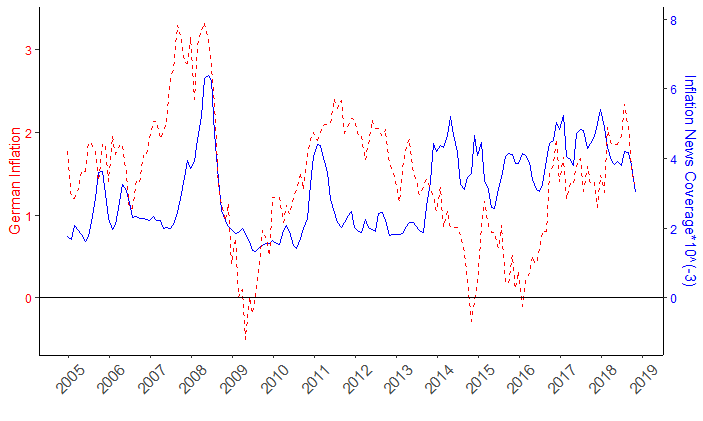
\includegraphics{Inflation_Count.png}
    \caption{Media Coverage and Inflation}
    \label{Inflation_Count}
\end{subfigure}
\hfil
\begin{subfigure}{6cm}
    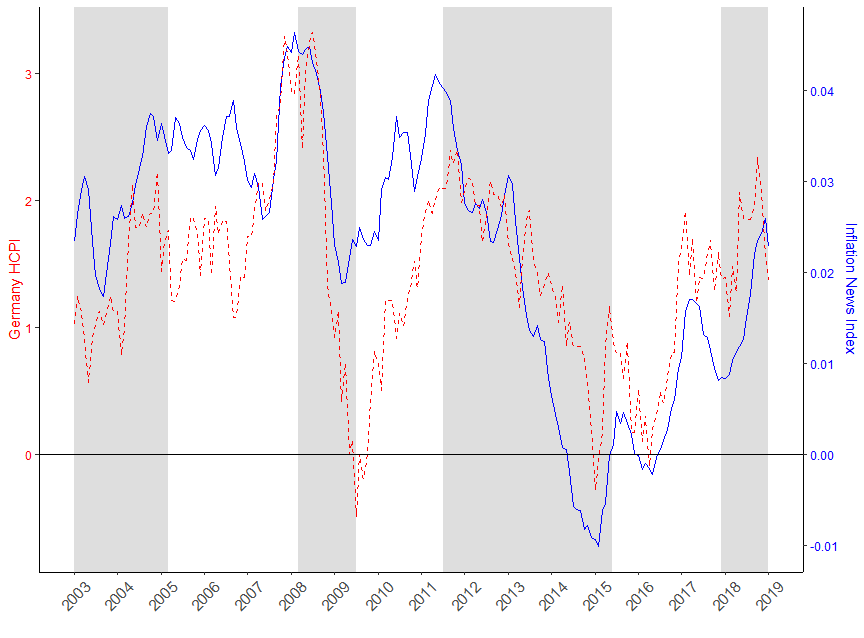
\includegraphics{Inflation_Sentiment_Direction.png}
    \caption{INI and Inflation}
    \label{Inflation_Sentiment_Direction}
\end{subfigure}
\caption{Media Reporting and Inflation: Figure (a) depicts the monthly year-on-year inflation for Germany in red and the media coverage in blue. Media coverage is defined as the number of inflation-related sentences divided by the total number of sentences to account for the varying number of articles in each year. Figure (b) depicts the monthly year-on-year inflation for Germany in red and the INI in blue.}
\label{fig:News Index}
    \end{figure}

%Figure~\ref{fig:ECB Index} depicts the three ECB indexes and corresponding macroeconomic variables. 
Figure~\ref{ECB_inf} illustrates the strong correlation between Eurozone inflation, the ECB inflation index, and the ECB staff inflation projection. In 2006, the ECB Inflation Index reached a peak near the height of the Great Recession, even though inflation during this period was relatively lower. Similarly to the INI, the low inflation experienced at the beginning of 2009 was accompanied by a considerably smaller dip in the ECB inflation index compared to the 2014 dip. In this case, the ECB inflation index led Eurozone inflation from 2011 to 2014.

   \begin{figure}[!ht]
    \centering
    \setkeys{Gin}{width=\linewidth,height=6cm} %set image parameters
%\begin{subfigure}{6cm}
%    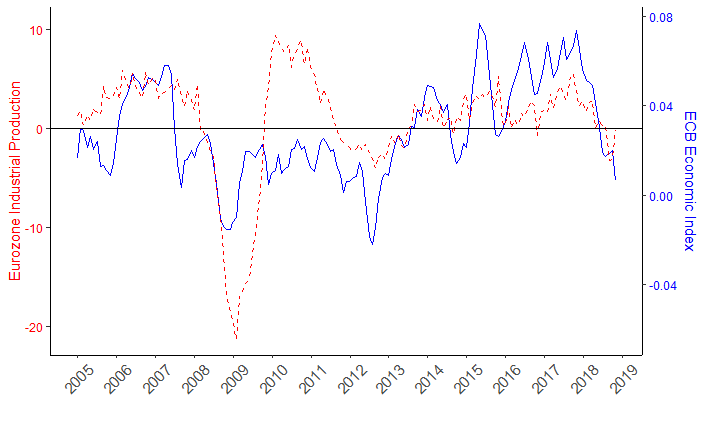
\includegraphics{ECB_eco_Industrial_prod.png}
%    \caption{ECB Economic Outlook}
%    \label{ECB_eco}
%\end{subfigure}
%\hfil
%\begin{subfigure}{6cm}
    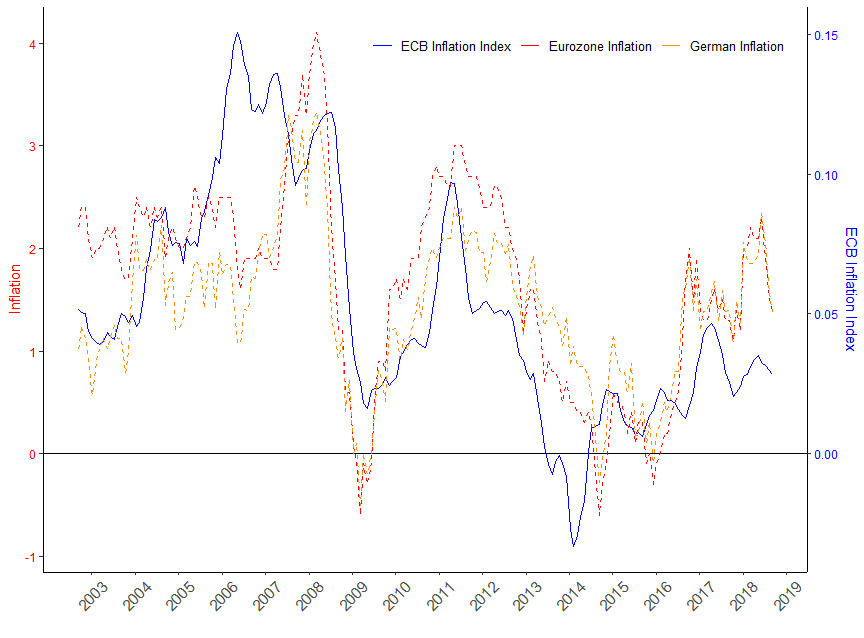
\includegraphics{ECB_inf_inf.png}
  %  \caption{ECB Inflation}
  \caption{The plot depicts the monthly year-on-year inflation in the Eurozone in red, alongside the ECB inflation index in blue.}
    \label{ECB_inf}
%\end{subfigure}
%\vfil
%\begin{subfigure}{6cm}
%    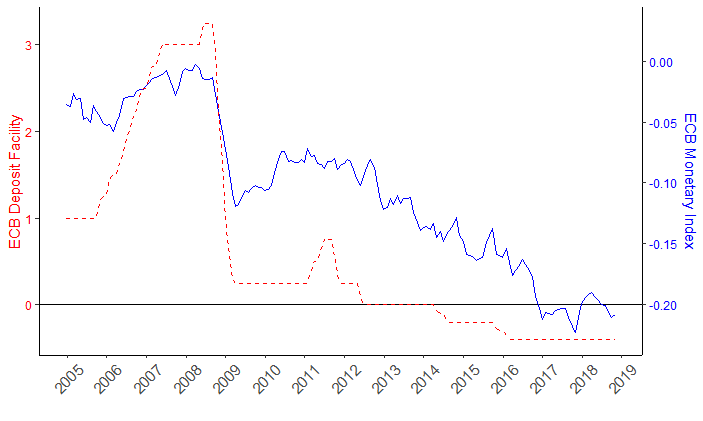
\includegraphics{ECB_mon_df.png}
%    \caption{ECB Monetary}
%    \label{ECB_mon}
%\end{subfigure}
%\caption{ECB Indices: Figure (a) depicts the monthly growth of industrial production in the Eurozone in red, alongside the Economic Outlook index in blue. Figure (b) depicts the monthly HICP growth for the Eurozone in red, in conjunction with the ECB inflation outlook index in blue. Figure (c) depicts the deposit facility rates in red, along with the monetary outlook index in blue.}
%\label{fig:ECB Index}
    \end{figure}
%\textcolor{red}{NOTE 1: Professional Forecaster Inflation Expectations are stronger correlated with ECB Inflation Index than with Inflation Expectations. Could be because of the European prof. Inf. Exp.}
%\\
%\textcolor{red}{NOTE 2: The results are quite similar to Picault et. al (2017) and Marozzi (2021), which is reassuring, but I only add 4 more years to the dataset. Therefore, my approach adds little new information regarding the ECB indices.}

Figure~\ref{Abs_exp_res} shows that media bias correlates with the media bias. Especially after the Great Recession the expectation gap and the media bias dropped and remained low until they increased again after 2014. 

%\cite{Carroll2003} define the inflation expectation error of households as the squared difference between the household inflation expectations and professional inflation expectations. \cite{LamlaLein2014} instead uses the absolute difference. Because I'm not only interested in the absolute size of the inflation gap, but also the direction 

%To measure the error, I use the EU household inflation expectation described in and the professional inflation forecasts for the Eurozone described in (SECTION 2). My interest lies in the deviation between the household inflation expectations from the optimal forecasts. Therefore, I follow Lamla (2014) and calculate the household forecast errors as the difference between the household inflation expectations and professional inflation forecast for the Eurozone in the coming 12 months. I deviate from Lamla (2014) by taking the non-absolute error. (CITE) and (CITE) show that households react differently to news regarding high and low inflation.

   \begin{figure}[!ht]
    \centering
    \setkeys{Gin}{width=\linewidth,height=6cm} %set image parameters
%\begin{subfigure}{6cm}
    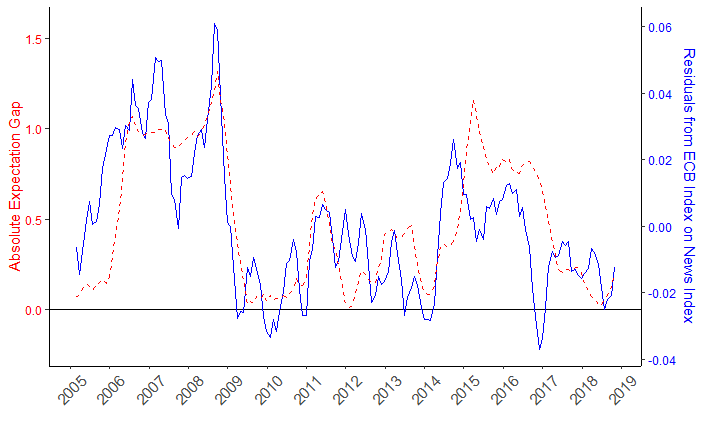
\includegraphics{abs_exp_res.png}
%    \caption{Absolute Expt. Gap}
\caption{The figure shows the absolute expectation gap between proffesional inflation forecasts and quantified household inflation expectations in red and the regression residuals from the ECB inflation index on the INI in blue.}
    \label{Abs_exp_res}
%\end{subfigure}
%\hfil
%\begin{subfigure}{6cm}
%    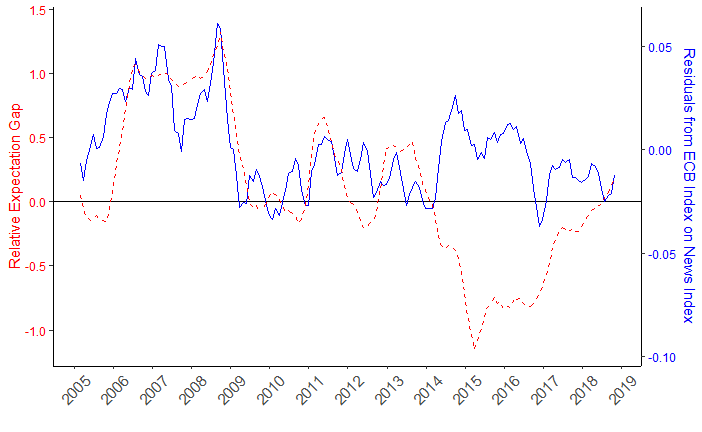
\includegraphics{rel_exp_res.png}
%    \caption{Relative Expt. Gap}
%    \label{Rel_exp_res}
%\end{subfigure}
%\vfil
%\begin{subfigure}{6cm}
%    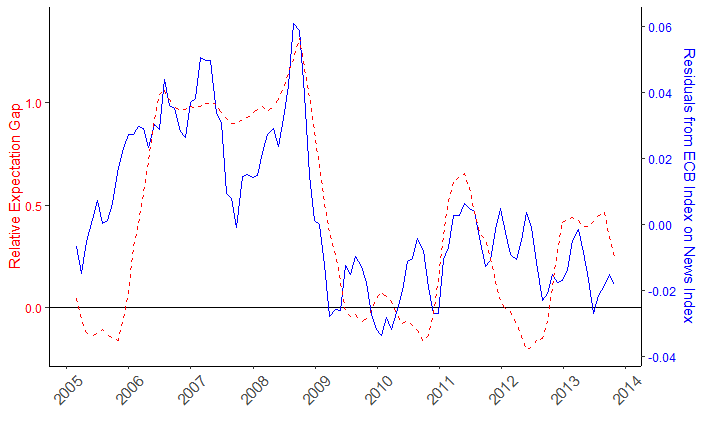
\includegraphics{rel_exp_res_prev2014.png}
%    \caption{Relative Expt. Gap - Before 2014}
%    \label{rel_exp_res_prev2014}
%\end{subfigure}
%\hfil
%\begin{subfigure}{6cm}
%    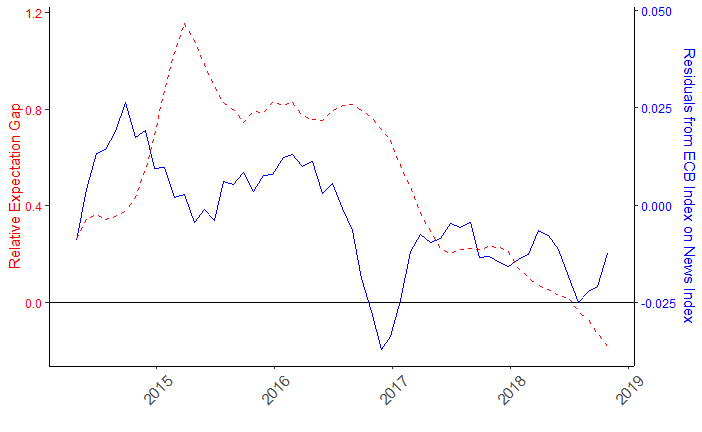
\includegraphics{rel_exp_res_aft2014.png}
%    \caption{Negative Relative Expt. Gap - After 2014}
%    \label{rel_exp_res_aft2014}
%\end{subfigure}
%\caption{Figure (a) shows the absolute expectation gap and regression residuals between the ECB inflation outlook and News inflation indices. Figure (b) presents the relative expectation gap and corresponding residuals. Figures (c) and (d) display the relative expectation gap for 2005-2014 and 2014-2018, respectively.}
%\label{fig:Expectation Gap}
    \end{figure}

\section{Econometric Framework}\label{sec:Econometric Framework}
To test my two hypothesis, I examine the impact of the media bias and media-central bank alignment on the inflation expectation error. To do this, I estimate the following equation
\\
$B_t = \beta_0 + \beta_1 \tilde{V_t} + \beta_2 \tilde{\alpha_t} + \beta_3 \tilde{\lambda_t} +\beta_3 \pi_{t-1} + \beta_4 B_{t-1} + \epsilon_t$ \\
where $\beta_0$ is a constant, $\tilde{V_t}$ is the share of inflation related sentences in the media divided by the number of all sentences,  $\tilde{\alpha_t}$ is the residual from the linear regression of the ECB inflation index on the INI and media coverage, $\tilde{\lambda_t}$ is the number of sentences in which the ECB is directly or indirectly cited divided by the number of all sentences. The equation is estimated via OLS using Newey-West standard errors.
%\\
%To avoid simultaneity issues I follow \cite{LamlaLein2014} In order to obtain media data for a given month, I aggregate the media reports for each month, excluding any articles which are potentially related to the consumer survey results in the month. Specifically, I sum up the media articles until the day before the consumer survey is released. The sentences from the summed up articles are then used to derive the news index and news count for the given month.
%\\
%\textcolor{red}{Andere finden die das ähnlich gemacht haben.}
%\\
\newpage
\section{Results}\label{sec:Results}

\begin{table}[!ht]
\centering 
  \caption{ECB - Stm} 
  \label{tab:ECB - Stm}
\begin{tabular}{l*{6}{c}}   
\toprule
                    & (1) & (2) & (3) & (4) & (5) \\
\midrule
$B_{t-1}$           &     & 0.032 & -0.019 & -0.035 & -0.077 \\
                    &     & (0.112) & (0.109) & (0.105) & (0.107) \\
$\pi_{t-1}$         &     & -0.005 & -0.016 & -0.023 & -0.032 \\
                    &     & (0.021) & (0.022) & (0.019) & (0.021) \\
$\tilde{V_t}$       & -7.290 & -7.613 & -16.667 & 5.391 & -4.107 \\
                    & (15.445) & (15.842) & (16.480) & (13.313) & (13.609) \\
$\tilde{\alpha_t}$  &     &     & 1.638* &     & 1.521* \\
                    &     &     & (0.873) &     & (0.824) \\
$\tilde{\lambda_t}$ &     &     &     & -3.624*** & -3.321*** \\
                    &     &     &     & (1.179) & (1.030) \\
$Constant$          & 0.254*** & 0.253*** & 0.281*** & 0.351*** & 0.369*** \\
                    & (0.033) & (0.051) & (0.057) & (0.053) & (0.058) \\
\midrule
$R^2$               & 0.004 & 0.005 & 0.101 & 0.088 & 0.170 \\
\bottomrule
\end{tabular} 
\parbox{0.8\textwidth}{\centering \small *** p $<$ 0.01, ** p $<$ 0.05, * p $<$ 0.1.}
\end{table}

\begin{table}[!ht]
\centering 
  \caption{ECB - Berk 1} 
  \label{tab:ECB - Berk 1}
\begin{tabular}{l*{6}{c}}   
\toprule
                    & (1) & (2) & (3) & (4) & (5) \\
\midrule
$B_{t-1}$           &     & 0.196** & 0.187** & 0.190** & 0.183** \\
                    &     & (0.088) & (0.086) & (0.092) & (0.091) \\
$\pi_{t-1}$         &     & -0.286*** & -0.290*** & -0.289*** & -0.293*** \\
                    &     & (0.040) & (0.039) & (0.040) & (0.041) \\
$\tilde{V_t}$       & -57.757 & -75.719*** & -78.287*** & -73.604*** & -76.451*** \\
                    & (42.787) & (25.444) & (25.221) & (25.929) & (25.463) \\
$\tilde{\alpha_t}$  &     &     & 0.507 &     & 0.493 \\
                    &     &     & (1.256) &     & (1.255) \\
$\tilde{\lambda_t}$ &     &     &     & -0.540 & -0.451 \\
                    &     &     &     & (1.404) & (1.396) \\
$Constant$          & 0.540*** & 0.837*** & 0.848*** & 0.854*** & 0.861*** \\
                    & (0.115) & (0.093) & (0.093) & (0.110) & (0.113) \\
\midrule
$R^2$               & 0.053 & 0.552 & 0.554 & 0.553 & 0.555 \\
\bottomrule
\end{tabular} 
\parbox{0.8\textwidth}{\centering \small *** p $<$ 0.01, ** p $<$ 0.05, * p $<$ 0.1.}
\end{table}

\begin{table}[!ht]
\centering 
  \caption{ECB - Berk 5} 
  \label{tab:ECB - Berk 5}
\begin{tabular}{l*{6}{c}}   
\toprule
                    & (1) & (2) & (3) & (4) & (5) \\
\midrule
$B_{t-1}$           &     & 0.463*** & 0.409*** & 0.371*** & 0.324*** \\
                    &     & (0.107) & (0.102) & (0.102) & (0.096) \\
$\pi_{t-1}$         &     & 0.072 & 0.061* & 0.056 & 0.047 \\
                    &     & (0.049) & (0.036) & (0.045) & (0.033) \\
$\tilde{V_t}$       & -56.125** & -25.989 & -41.558*** & -14.878 & -30.443** \\
                    & (25.206) & (17.162) & (14.396) & (14.779) & (12.348) \\
$\tilde{\alpha_t}$  &     &     & 2.203** &     & 2.113*** \\
                    &     &     & (0.865) &     & (0.799) \\
$\tilde{\lambda_t}$ &     &     &     & -4.666*** & -4.401*** \\
                    &     &     &     & (0.964) & (0.820) \\
$Constant$          & 0.455*** & 0.137** & 0.177*** & 0.273*** & 0.304*** \\
                    & (0.064) & (0.055) & (0.055) & (0.050) & (0.050) \\
\midrule
$R^2$               & 0.089 & 0.397 & 0.468 & 0.448 & 0.513 \\
\bottomrule
\end{tabular} 
\parbox{0.8\textwidth}{\centering \small *** p $<$ 0.01, ** p $<$ 0.05, * p $<$ 0.1.}
\end{table}

\begin{table}[!ht]
\centering 
  \caption{ECB - Quant} 
  \label{tab:ECB - Quant}
\begin{tabular}{l*{6}{c}}   
\toprule
                    & (1) & (2) & (3) & (4) & (5) \\
\midrule
$B_{t-1}$           &     & 0.362 & 0.375 & 0.289 & 0.305 \\
                    &     & (0.641) & (0.539) & (0.545) & (0.447) \\
$\pi_{t-1}$         &     & 0.247 & 0.174 & 0.189 & 0.129 \\
                    &     & (0.394) & (0.346) & (0.341) & (0.308) \\
$\tilde{V_t}$       & 121.867 & 312.588 & 270.628 & 375.381 & 335.130 \\
                    & (552.031) & (290.579) & (268.372) & (281.803) & (273.899) \\
$\tilde{\alpha_t}$  &     &     & 7.704* &     & 6.691* \\
                    &     &     & (4.363) &     & (3.644) \\
$\tilde{\lambda_t}$ &     &     &     & -26.143** & -24.557** \\
                    &     &     &     & (10.258) & (10.015) \\
$Constant$          & 2.550*** & 1.130 & 1.200 & 1.817* & 1.837** \\
                    & (0.644) & (1.110) & (1.018) & (0.982) & (0.843) \\
\midrule
$R^2$               & 0.019 & 0.266 & 0.310 & 0.355 & 0.388 \\
\bottomrule
\end{tabular} 
\parbox{0.8\textwidth}{\centering \small *** p $<$ 0.01, ** p $<$ 0.05, * p $<$ 0.1.}
\end{table}

\newpage


\section{Conclusions} \label{sec:Conclusions}

%\section*{References}

\bibliography{mybibfile}

\newpage

\appendix

\section{Quantification of Inflation Expectations}\label{sec:Quantification_of_Inflation_Expectations}

The European Commission's Business and Consumer Survey consumers are asked if they expect prices to fall, stay the same, increase slower than before, increase at the same rate or increase at a higher rate in the coming 12 months and in the last 12 months. 
\\
I use the rolling-window-regression approach by \cite{Lahiri2015} which is based on an extended version of the Carlson-Parkin method \citep{Carlson1975} by \cite{Berk1999}. The extended version of \cite{Berk1999} does not impose unbiasedness of inflation expectations. Instead the current perceived inflation rate is directly linked to the expected inflation rate.  
\\
By assumption each responded i forms a subjective probability distribution for individuals percentage price changes $y_{it}$ over the next twelve months. Let $f_i(y{_it})$ be the subjective probability distribution with mean $\mu_{it}$ and variance $\sigma_{it}$. Following \cite{Batchelor1988} method assumes for a survey with five possible answers that the respondent answers prices in the future increase, increase at the same rate, increase at a slower rate, stay the same or fall according as $ y_{it} < - \delta_{it}^L, - \delta_{it}^L < y_{it} < \delta_{it}^U , \delta_{it}^L < y_{it} < \delta_{it}^U,  \delta_{it}^U < y_{it} < \lambda_{it}, \lambda_{it} < y_{it}$ \textcolor{red}{Nochmal überprüfen, Ist Notation von \cite{Batchelor1988} besser?}. Based on the survey responses the corresponding aggregate probabilities can be formulated as $P(y <  -\delta_{it}^L) = A_t, P(y < \delta_{it}^U) - P(y > - \delta_{it}^L) = B_t, P(y < \delta_{it}^U) - P(y > \delta_{it}^L) = C_t, P(y < \lambda_{it}) - P(y > \delta_{it}^U) = D_t.$ I denote $a_t, b_t, c_t$ and $ d_t$ the abscissae of the standard logistical distribution function corresponding to the cumulative probabilities $A_t, \ A_t + B_t, \ A_t + B_t + C_t$ and $A_t + B_t + C_t + D_t$. The mean expected inflation rate $\mu_t = E_t \pi_{t+12}$ can then be formulated as 
\begin{align*}
\mu_t = \lambda_t \frac{(a_t + b_t)}{(a_t + b_t - c_t - d_t)}
\end{align*}
Similarly, I denote $a_t\sp{\prime}, b_t\sp{\prime}, c_t\sp{\prime}$ and $ d_t\sp{\prime}$ as the abscissae of the standard logistical distribution function for the perceived inflation. Assuming that the response threshold $\lambda_{it}$ \textcolor{red}{Nochmal überprüfen} is the same for expected and perceived inflation, the perceived inflation can be formulated as 
\begin{align*}
\mu_t\sp{\prime} = \lambda_t \frac{(a_t\sp{\prime} + b_t\sp{\prime})}{(a_t\sp{\prime} + b_t\sp{\prime} - c_t\sp{\prime} - d_t\sp{\prime})}
\end{align*}
For the choice of the scaling parameter $\lambda_t$ I use the rolling window based regression by \cite{Lahiri2015}. Following \cite{Rosenblatt-Wisch2015} running the regression
\begin{align*}
\pi_t = \lambda \frac{(a_t\sp{\prime} + b_t\sp{\prime})}{(a_t\sp{\prime} + b_t\sp{\prime} - c_t\sp{\prime} - d_t\sp{\prime})} + u_t 
\end{align*}
using a sample window of $t - w + 1 to t$ implies
\begin{align*}
\hat{\lambda_t} = \frac{\sum^t_{k = t-w+1}(a_t\sp{\prime} + b_t\sp{\prime})/(a_t\sp{\prime} + b_t\sp{\prime} - c_t\sp{\prime} - d_t\sp{\prime})\pi_t}{\sum^t_{k = t-w+1}(a_t\sp{\prime} + b_t\sp{\prime})/((a_t\sp{\prime} + b_t\sp{\prime} - c_t\sp{\prime} - d_t\sp{\prime}))^2}
\end{align*}
where $w$ is the size of the rolling window. \cite{Lahiri2015} choose $w$ as nine years for the inflation expectations of the Michigan Consumer Survey. I follow \cite{Lahiri2015} and also choose nine years for $w$. The resulting household inflation expectations and the professional inflation expectations are shown in figure~\ref{fig:Inflation Expectations}.
\\
\textcolor{red}{Robustness Check for different windows?}
\\
\textcolor{red}{TO CLOSE TO Rosenblatt-Wisch and Scheufele 2014??}

   \begin{figure}[!ht]
    \centering
    \setkeys{Gin}{width=\linewidth,height=6cm} %set image parameters
\begin{subfigure}{6cm}
    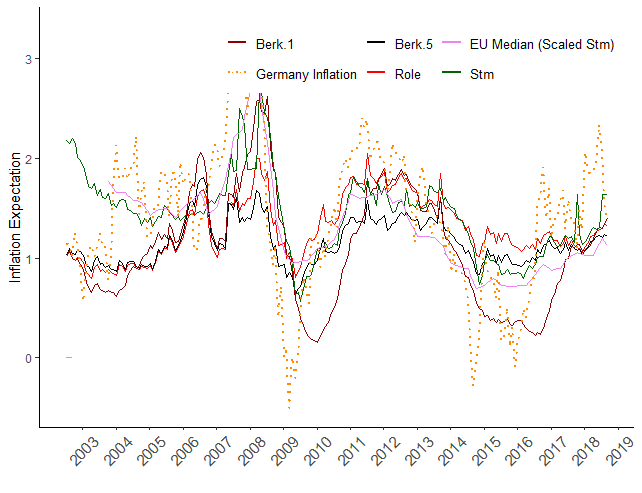
\includegraphics{Household_Inf_Exp.png}
    \caption{Household Inflation Expectations}
    \label{Inflation_Count}
\end{subfigure}
\hfil
\begin{subfigure}{6cm}
    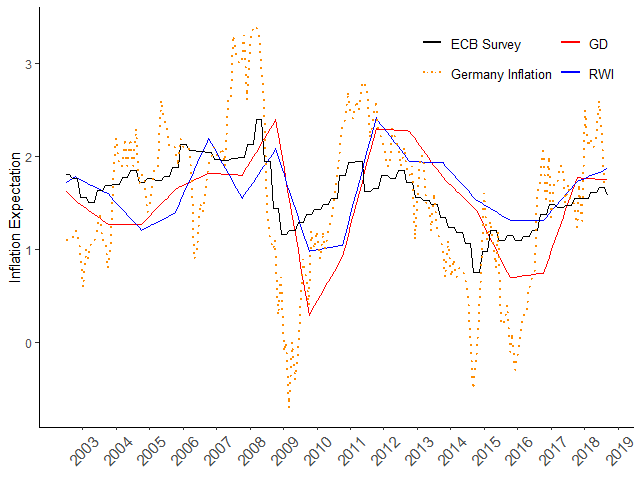
\includegraphics{Prof_Inf_Exp.png}
    \caption{Professional Inflation Expectations}
    \label{Inflation_Sentiment_Direction}
\end{subfigure}
\caption{Inflation Expectations.}
\label{fig:News Index}
    \end{figure}

%  \begin{figure}[!ht]
%    \centering
%    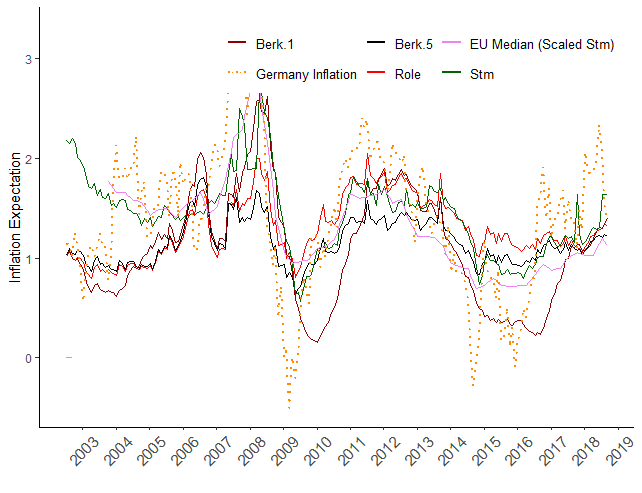
\includegraphics{Household_Inf_Exp.png}
%    \caption{Household Inflation Expectations}
%    \end{figure}
%\label{fig:Inflation Expectations}

\section{Alternative Survey Quantification Methods and Professional Forecasts}

\begin{table}[!ht]
\centering 
  \caption{Inflation Expectation Gap: RWI - Stm} 
  \label{tab:Inflation Expectation Gap}
\begin{tabular}{l*{6}{c}}   
\toprule
                    & (1) & (2) & (3) & (4) & (5) \\
\midrule
$B_{t-1}$           &     & 0.052 & 0.057 & 0.041 & 0.047 \\
                    &     & (0.126) & (0.125) & (0.129) & (0.128) \\
$\pi_{t-1}$         &     & 0.103** & 0.102** & 0.108*** & 0.107*** \\
                    &     & (0.043) & (0.043) & (0.040) & (0.041) \\
$\tilde{V_t}$       & 41.134* & 48.032*** & 47.606*** & 43.221** & 42.613** \\
                    & (22.475) & (18.037) & (18.098) & (18.726) & (18.753) \\
$\tilde{\alpha_t}$  &     &     & 0.111 &     & 0.138 \\
                    &     &     & (0.721) &     & (0.722) \\
$\tilde{\lambda_t}$ &     &     &     & 1.136 & 1.155 \\
                    &     &     &     & (1.355) & (1.344) \\
$Constant$          & 0.340*** & 0.176** & 0.176** & 0.156** & 0.155** \\
                    & (0.052) & (0.081) & (0.082) & (0.077) & (0.078) \\
\midrule
$R^2$               & 0.067 & 0.190 & 0.190 & 0.194 & 0.195 \\
\bottomrule
\end{tabular} 
\parbox{0.8\textwidth}{\centering \small *** p $<$ 0.01, ** p $<$ 0.05, * p $<$ 0.1.}
\end{table}

\begin{table}[!ht]
\centering 
  \caption{Inflation Expectation Gap: RWI - Berk 1} 
  \label{tab:Inflation Expectation Gap}
\begin{tabular}{l*{5}{c}}   
\toprule
                    & (1) & (2) & (3) & (4) & (5) \\
\midrule
$B_{t-1}$           &     & 0.155 & 0.131 & 0.140 & 0.123 \\
                    &     & (0.283) & (0.257) & (0.234) & (0.211) \\
$\pi_{t-1}$         &     & -0.140** & -0.139** & -0.121* & -0.121* \\
                    &     & (0.068) & (0.066) & (0.065) & (0.063) \\
$\tilde{V_t}$       & 25.468 & 5.626 & 9.958 & -14.568 & -10.634 \\
                    & (32.896) & (40.084) & (38.428) & (39.098) & (37.603) \\
$\tilde{\alpha_t}$  &     &     & -0.820 &     & -0.635 \\
                    &     &     & (1.516) &     & (1.508) \\
$\tilde{\lambda_t}$ &     &     &     & 4.931*** & 4.791*** \\
                    &     &     &     & (1.634) & (1.584) \\
$Constant$          & 0.592*** & 0.702*** & 0.714*** & 0.609*** & 0.621*** \\
                    & (0.119) & (0.229) & (0.207) & (0.222) & (0.201) \\
\midrule
$R^2$               & 0.013 & 0.199 & 0.206 & 0.241 & 0.245 \\
\bottomrule
\end{tabular} 
\parbox{0.8\textwidth}{\centering \small *** p $<$ 0.01, ** p $<$ 0.05, * p $<$ 0.1.}
\end{table}

\begin{table}[!ht]
\centering 
  \caption{Inflation Expectation Gap: RWI - Berk 5} 
  \label{tab:Inflation Expectation Gap}
\begin{tabular}{l*{5}{c}}   
\toprule
                    & (1) & (2) & (3) & (4) & (5) \\
\midrule
$B_{t-1}$           &     & -0.132 & -0.152 & -0.139 & -0.156 \\
                    &     & (0.192) & (0.186) & (0.186) & (0.185) \\
$\pi_{t-1}$         &     & 0.158*** & 0.162*** & 0.167*** & 0.170*** \\
                    &     & (0.045) & (0.042) & (0.042) & (0.041) \\
$\tilde{V_t}$       & -39.960 & -31.620 & -29.295 & -40.853 & -38.112 \\
                    & (33.795) & (25.727) & (24.489) & (26.275) & (24.478) \\
$\tilde{\alpha_t}$  &     &     & -0.746 &     & -0.669 \\
                    &     &     & (1.338) &     & (1.340) \\
$\tilde{\lambda_t}$ &     &     &     & 2.133 & 1.982 \\
                    &     &     &     & (1.632) & (1.550) \\
$Constant$          & 0.485*** & 0.323** & 0.328** & 0.282** & 0.289** \\
                    & (0.086) & (0.135) & (0.135) & (0.138) & (0.138) \\
\midrule
$R^2$               & 0.044 & 0.296 & 0.304 & 0.307 & 0.314 \\
\bottomrule
\end{tabular} 
\parbox{0.8\textwidth}{\centering \small *** p $<$ 0.01, ** p $<$ 0.05, * p $<$ 0.1.}
\end{table}

\begin{table}[!ht]
\centering 
  \caption{Inflation Expectation Gap: GD - Stm} 
  \label{tab:Inflation Expectation Gap}
\begin{tabular}{l*{5}{c}}   
\toprule
                    & (1) & (2) & (3) & (4) & (5) \\
\midrule
$B_{t-1}$           &     & 0.112 & 0.016 & 0.110 & 0.016 \\
                    &     & (0.149) & (0.144) & (0.149) & (0.145) \\
$\pi_{t-1}$         &     & 0.071 & 0.083* & 0.072 & 0.083* \\
                    &     & (0.054) & (0.045) & (0.054) & (0.045) \\
$\tilde{V_t}$       & -25.775 & -18.217 & -14.263 & -19.757 & -14.424 \\
                    & (17.555) & (16.962) & (15.559) & (18.211) & (16.574) \\
$\tilde{\alpha_t}$  &     &     & -1.782*** &     & -1.781*** \\
                    &     &     & (0.567) &     & (0.571) \\
$\tilde{\lambda_t}$ &     &     &     & 0.353 & 0.036 \\
                    &     &     &     & (1.397) & (1.440) \\
$Constant$          & 0.325*** & 0.188** & 0.202*** & 0.181** & 0.202*** \\
                    & (0.047) & (0.079) & (0.075) & (0.080) & (0.077) \\
\midrule
$R^2$               & 0.029 & 0.104 & 0.169 & 0.105 & 0.169 \\
\bottomrule
\end{tabular} 
\parbox{0.8\textwidth}{\centering \small *** p $<$ 0.01, ** p $<$ 0.05, * p $<$ 0.1.}
\end{table}

\begin{table}[!ht]
\centering 
  \caption{Inflation Expectation Gap: GD - Berk 1} 
  \label{tab:Inflation Expectation Gap}
\begin{tabular}{l*{6}{c}}   
\toprule
                    & (1) & (2) & (3) & (4) & (5) \\
\midrule
$B_{t-1}$           &     & 0.193 & 0.180 & 0.164 & 0.155 \\
                    &     & (0.176) & (0.176) & (0.182) & (0.183) \\
$\pi_{t-1}$         &     & 0.040 & 0.043 & 0.052 & 0.053 \\
                    &     & (0.038) & (0.038) & (0.032) & (0.033) \\
$\tilde{V_t}$       & -2.105 & -2.325 & -0.318 & -15.398 & -13.481 \\
                    & (18.141) & (19.385) & (18.836) & (19.883) & (19.435) \\
$\tilde{\alpha_t}$  &     &     & -0.504 &     & -0.393 \\
                    &     &     & (1.030) &     & (0.995) \\
$\tilde{\lambda_t}$ &     &     &     & 3.171* & 3.085* \\
                    &     &     &     & (1.644) & (1.639) \\
$Constant$          & 0.442*** & 0.301** & 0.303** & 0.249** & 0.252** \\
                    & (0.053) & (0.120) & (0.125) & (0.113) & (0.115) \\
\midrule
$R^2$               & 0.0002 & 0.037 & 0.044 & 0.081 & 0.085 \\
\bottomrule
\end{tabular} 
\parbox{0.8\textwidth}{\centering \small *** p $<$ 0.01, ** p $<$ 0.05, * p $<$ 0.1.}
\end{table}

\begin{table}[!ht]
\centering 
  \caption{GD - Berk 5} 
  \label{tab:GD - Berk 5}
\begin{tabular}{l*{6}{c}}   
\toprule
                    & (1) & (2) & (3) & (4) & (5) \\
\midrule
$B_{t-1}$           &     & 0.032 & -0.015 & 0.031 & -0.015 \\
                    &     & (0.126) & (0.122) & (0.128) & (0.122) \\
$\pi_{t-1}$         &     & 0.204*** & 0.215*** & 0.207*** & 0.216*** \\
                    &     & (0.059) & (0.058) & (0.059) & (0.058) \\
$\tilde{V_t}$       & -34.755 & -21.298 & -17.411 & -24.066 & -18.831 \\
                    & (25.552) & (18.306) & (17.546) & (19.283) & (18.434) \\
$\tilde{\alpha_t}$  &     &     & -1.420 &     & -1.407 \\
                    &     &     & (1.008) &     & (1.023) \\
$\tilde{\lambda_t}$ &     &     &     & 0.651 & 0.325 \\
                    &     &     &     & (1.311) & (1.284) \\
$Constant$          & 0.470*** & 0.165** & 0.173** & 0.152** & 0.166** \\
                    & (0.082) & (0.071) & (0.069) & (0.074) & (0.069) \\
\midrule
$R^2$               & 0.034 & 0.381 & 0.409 & 0.382 & 0.409 \\
\bottomrule
\end{tabular} 
\parbox{0.8\textwidth}{\centering \small *** p $<$ 0.01, ** p $<$ 0.05, * p $<$ 0.1.}
\end{table}


\section{Additional Rules for Lexicon Text Classification}\label{sec:Additional Rules for Lexicon Text Classification}

\end{document}